\documentclass[conference]{IEEEtran}
\usepackage{times}
\usepackage[numbers]{natbib}
\usepackage{multicol}
\usepackage[bookmarks=true]{hyperref}
\usepackage{graphicx}
\usepackage{booktabs}
\usepackage{amsmath}
\usepackage{tikz}
\usetikzlibrary{positioning,arrows.meta,fit}

% RSS 2027 Stage 1 (extended abstract): at most 5 pages of content + 1 page of references, anonymised.
% Draft, 2026-11-13. Every number traces to an F-number in results/findings.md; see paper/rss2027/README.md.

\ifx\pdfinfo\undefined\else % pdfLaTeX (the submission engine); skipped under XeTeX, used only for length checks
\pdfinfo{
   /Title  (Learned Whole-Body Control Through a Nine-Hertz Arm)
   /Subject (Robotics)
   /Keywords (legged manipulation; whole-body control; sim-to-real; force control; actuator interfaces)
}
\fi

\newcommand{\hyp}[1]{\textbf{H#1}}

\begin{document}

\title{Learned Whole-Body Control Through a Nine-Hertz Arm:\\
Interface Identification for Force-Aware Loco-Manipulation\\ on a Low-Cost Quadruped Manipulator}

\author{Author Names Omitted for Anonymous Review}

\maketitle

\begin{abstract}
Learned whole-body controllers for legged manipulators assume an arm whose joints are commanded at the policy rate.
The arms commonly sold for low-cost quadrupeds do not offer this. They are bus-servo arms behind closed firmware that
accept joint setpoints at about 10\,Hz and report their angles at 9\,Hz. We ask what such an interface does to a learned,
force-aware whole-body policy, and what must be identified to deploy one. Our hypothesis is that the transfer gap is set by
two interfaces rather than by the arm's dynamics: the arm's command--report timing, and how far the real legs follow their
targets under low-gain joint control. We propose to identify both from the robot's own logs and to close each at the
interface, leaving the policy architecture unchanged. Preliminary results on a Unitree Go2 with a D1 arm support
parts of this. A 0.3--0.7\,s arm stall turns out to be set by where a command lands in the report cycle, not by the
command rate, and locking one command to each report removes it (52 skipped reports in 590 held cycles against 0 in 716;
29.7\% of a six-joint motion lost against 0.8\%). A slew-and-lag model fitted to the reports predicts held-out motion
to 0.2--0.6$^\circ$ RMS. A policy that tracked to 1.9\,cm on an idealized arm degrades to 16.6\,cm on this model.
The first policy that tracks on the model still failed on the robot within 1.5\,s, because the real legs move 0.17 of
their commanded motion. After retraining against sticky legs and screening on replayed real frames, the policy reached
goals 30\,cm away, held its hand while walking for 30\,s, and wiped a bench. Its trained force input raised the
measured contact force from 7 to 19\,N, open loop. We state four falsifiable hypotheses and the experiments that test them.
\end{abstract}

\IEEEpeerreviewmaketitle

%------------------------------------------------------------------------------
\section{Introduction}

Reinforcement-learned whole-body controllers now let a legged robot use its body to extend, steady and push with an
attached arm \citep{fu2022deep, liu2024visual, ha2024umi, portela2024learning, zhi2025unified, liu2026mlm}. These systems share an assumption that is easy to
miss: the arm is a fast, transparent actuator. Its joints take a new position or torque target every policy step
(typically 50\,Hz) and are servoed by a kilohertz PD loop that the simulator reproduces. The policy can then use its arm
targets as it uses its leg targets, as a continuous push whose effect it learns.

The arms sold as add-ons for low-cost quadrupeds break this assumption. The arm in this study is the Unitree D1, a
six-joint bus-servo arm offered as an accessory for the Go2. It accepts joint setpoints over DDS through closed firmware
that plans a motion to each one, and it reports its joint angles at 9.00\,Hz (one report every 111\,ms). There is no
higher-rate mode to unlock and no holding brake. Low-cost arms have widened access to manipulation research
\citep{zhao2023learning}, yet the learned whole-body control literature, as far as we can tell, does not ask what a policy should do when its arm is
a slow black box, or how one would know that a policy is ready for it.

This paper studies that question on a Go2 with a welded D1, using a released force-aware whole-body method
\citep{zhi2025unified} retrained in Isaac Lab \citep{mittal2023orbit}. Our central claim is that \emph{the transfer gap is set by
interfaces, not by the arm's dynamics}. Two interfaces matter. The first is the arm's command--report timing. The second
is how far the real legs follow their targets under the low PD gains that learned locomotion policies use. Each can be
identified from logs the robot already produces. Each can be closed where it occurs, by how commands are sent, by what
the policy trains against, and by what it is screened on before it runs, without a new policy architecture. The
contributions we propose to establish are:
\begin{enumerate}
\item an identification of a report-cycle stall in a commercial servo arm, and a report-locked command scheme that
removes it, with a two-parameter arm model fitted to 9\,Hz reports alone (\hyp{1});
\item evidence that a whole-body policy trained on an idealized arm is unusable on such an interface, that it can be
fine-tuned to work, and that the metric to watch is the command stream the arm receives, not tracking error (\hyp{2});
\item the finding that leg responsiveness is a second, hidden interface, together with a screen that replays recorded
real proprioception with the arm in closed loop and a matched test of whether it predicts deployment better than
simulation does (\hyp{3});
\item real-robot evidence that the policy's trained force input survives the interface as a monotone, open-loop force
command, and a test of closing the loop on proprioceptive force estimates (\hyp{4}).
\end{enumerate}
We regard a negative outcome for any of these as informative. If, for example, a decoupled controller with the same
interface layer matches the learned whole-body policy, then the interface work is what transfers, not the whole-body
learning, and we will report it that way (Sec.~\ref{sec:plan}).

%------------------------------------------------------------------------------
\section{Related Work}

\textbf{Learned whole-body loco-manipulation.} Unified policies for a legged base and arm
\citep{fu2022deep, liu2024visual, ha2024umi, liu2026mlm, hu2026tacloco} and force-aware or compliant extensions
\citep{portela2024learning, zhi2025unified, xu2025facet} command the arm at the policy rate, including on the Go2 with
low-cost arms \citep{liu2026mlm, hu2026tacloco}. With a D1 on a Go2, \citet{schperberg2026safe} learn only the legs and
control the arm with a model-based admittance law, reporting a 40\,Hz send/receive limit for the arm. Through the
vendor DDS interface we use, the same arm model reports at 9\,Hz (Sec.~\ref{sec:platform}); E1 tests where the
difference lies. Model-based whole-body
controllers make the same assumption at higher rates \citep{bellicoso2019alma, sleiman2021unified}. Decoupled designs combine a
learned locomotion policy with model-based arm control \citep{ma2022combining}. We reuse UniFP's formulation
\citep{zhi2025unified} unchanged and vary only what it is trained and screened against.

\textbf{Actuator and latency modelling for transfer.} Learned actuator networks \citep{hwangbo2019learning}, latency and
actuator modelling \citep{tan2018sim}, servo models for low-cost bus-servo robots \citep{yu2019sim, haarnoja2024learning}, dynamics randomization \citep{peng2018sim, rudin2022learning} and online adaptation
\citep{kumar2021rma} address actuators that are fast and observed at the control rate. Here the actuator is observed
about five times slower than the policy runs, through firmware with its own planner. Its dominant failure is a timing
interaction between command and report, not a torque--speed relation.

\textbf{Predicting real performance before deployment.} Simulation has been used as a proxy for real-world policy
evaluation \citep{li2024evaluating}. Our replay screen goes the other way: it keeps the real robot's recorded leg and body
states and closes only the arm through the identified interface.

%------------------------------------------------------------------------------
\section{Platform, Policy and Interfaces}
\label{sec:platform}

\textbf{Robot.} A Unitree Go2 carries a 3.15\,kg Unitree D1 (six revolute joints and a parallel gripper) on its expansion
rails. The legs are commanded at 50\,Hz through the low-level joint interface at $k_p{=}25$, $k_d{=}0.5$. The arm is
commanded over the vendor's DDS interface from the onboard computer. We measured the arm's interface on hardware. It reports joint angles at
9.00\,Hz. Its joints slew at 1.2--1.3\,rad/s. The firmware ignores a command without a gripper angle, and plans each new
setpoint from rest, so a stream of setpoints moves the arm well below its single-command speed. Releasing torque drops the
arm, because it has no brake, so every stop must keep it energized.

\textbf{Policy.} We use UniFP's force-aware whole-body formulation \citep{zhi2025unified} on the Go2+D1. One actor outputs 18 joint
targets at 50\,Hz: 12 for the legs and 6 for the arm. It is commanded a base velocity, a tool-tip position goal in a
yaw-aligned body frame, and a tool force of up to $\pm$8\,N. The force command enters the reward as a position offset of the
goal (5\,mm per newton in free space), and a history encoder is trained to estimate the external force. We
reimplemented the task in Isaac Lab (it matches the original Isaac Gym task term by term to within 0.4\%) and trained it
natively: 4,096 environments, 60,000 PPO \citep{schulman2017proximal} iterations. On a frozen validation set its
checkpoints reach a median quiet goal error of 1.6--2.4\,cm with no falls, on an \emph{idealized} arm, i.e., targets
sent to a PD drive every step. Later fine-tunes (2,048 environments, a few thousand iterations each) keep the architecture, observations and force
curriculum. They change only the arm and leg models, and add the penalties named below.

\textbf{The two interfaces.} Fig.~\ref{fig:system} shows the deployed loop. On the arm side, the policy's 50\,Hz targets
pass through a \emph{Follower}, which caps each joint's commanded speed at 45$^\circ$/s. A \emph{ReportClock} then sends one setpoint per angle report. On the leg side, the policy's targets go directly to
the joint PD. A monitor stops the run on a sustained arm lead (25$^\circ$ held 0.5\,s), leg-target bounds, tilt, or a
stale feed. A lead or command-step stop holds the arm energized, folds it and lies the robot down. A tilt, leg-bound or
feed fault damps every motor.

\begin{figure}[t]
\centering
\resizebox{\columnwidth}{!}{%
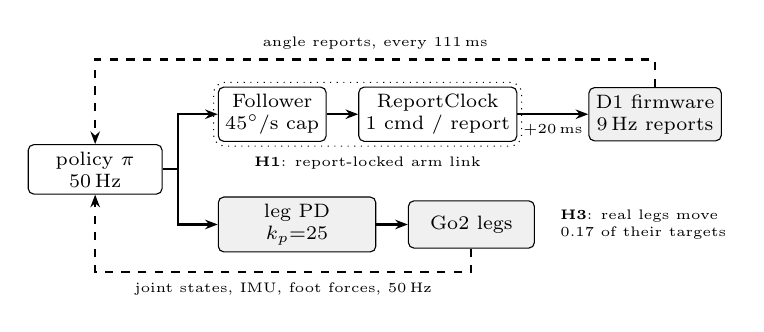
\begin{tikzpicture}[font=\scriptsize, node distance=3mm and 4mm,
  box/.style={draw, rounded corners=2pt, align=center, inner sep=2.5pt, minimum height=6mm},
  hw/.style={box, fill=black!6}, arr/.style={-{Stealth[length=1.6mm]}, thick}]
\node[box, minimum width=17mm] (pi) {policy $\pi$\\50\,Hz};
\node[box, right=7mm of pi, yshift=7mm] (fol) {Follower\\45$^\circ$/s cap};
\node[box, right=4mm of fol] (clk) {ReportClock\\1 cmd / report};
\node[hw, right=9mm of clk] (arm) {D1 firmware\\9\,Hz reports};
\node[hw, right=7mm of pi, yshift=-7mm, minimum width=20mm] (pd) {leg PD\\$k_p{=}25$};
\node[hw, right=4mm of pd, minimum width=16mm] (legs) {Go2 legs};
\draw[arr] (pi.east) -- ++(2mm,0) |- (fol.west);
\draw[arr] (pi.east) -- ++(2mm,0) |- (pd.west);
\draw[arr] (fol) -- (clk);
\draw[arr] (clk) -- node[below, font=\tiny]{+20\,ms} (arm);
\draw[arr] (pd) -- (legs);
\draw[arr, dashed] (arm.north) -- ++(0,3.5mm) -| node[above, pos=0.25, font=\tiny]{angle reports, every 111\,ms} (pi.north);
\draw[arr, dashed] (legs.south) -- ++(0,-3mm) -| node[below, pos=0.25, font=\tiny]{joint states, IMU, foot forces, 50\,Hz} (pi.south);
\node[draw, dotted, rounded corners, fit=(fol)(clk), inner sep=1.5pt] (h1) {};
\node[font=\tiny, anchor=north] at (h1.south) {\hyp{1}: report-locked arm link};
\node[font=\tiny, anchor=west, align=left] at ([xshift=2mm]legs.east) {\hyp{3}: real legs move\\0.17 of their targets};
\end{tikzpicture}}
\caption{Deployed loop. The arm is reached only through the report cycle (\hyp{1}). In training, the D1 block is
replaced by the identified slew--lag model (\hyp{2}), and the leg block by joints with randomized friction (\hyp{3}).}
\label{fig:system}
\end{figure}

%------------------------------------------------------------------------------
\section{Hypotheses}
\label{sec:hyp}

\hyp{1} \emph{Phase, not rate.} For an arm whose firmware handles setpoints against its own report cycle, lost reports are
caused by where a command lands in that cycle. One setpoint per report, at a fixed offset outside the critical
window, removes the loss with no drop in command throughput, and the arm's motion under such a stream can be identified
from its reports alone. \emph{Falsified if} locked streams lose reports at a rate not clearly below the unlocked stream's,
or if losses outside the window are comparable to those inside it.

\hyp{2} \emph{Train through the interface, and score what the arm receives.} A policy trained on an idealized arm uses
its arm targets as forces. On a slow position interface it does not track, and no rate limiter added at run time
fixes this. Fine-tuning against the identified model recovers tracking, but only if the policy is penalized on the
command stream the arm actually receives. \emph{Falsified if} the idealized policy, deployed through the same
Follower, tracks as well on hardware as the interface-trained one, or if the real hand error of the interface-trained
policy falls outside the distribution its simulation predicts.

\hyp{3} \emph{The legs are the second interface.} Under low-gain joint control, the real legs follow a much smaller
fraction of their commanded motion than simulated legs do. A policy that leans on its legs then winds up its arm instead.
Randomizing leg response in training makes such policies deployable. A screen that replays recorded real
proprioception with only the arm in closed loop ranks checkpoints for deployment better than simulation metrics do.
\emph{Falsified if} the replay's ranking of checkpoints correlates no better with their real outcomes than the simulator's
ranking does.

\hyp{4} \emph{The force channel survives as an open-loop command, and can be closed proprioceptively.} Through the same
interface, the trained force input produces a monotone, approximately affine contact force. A foot-force sum taken at the
same pose estimates that force well enough to close a slow outer loop. \emph{Falsified if} the real force is not monotone
in the command, or if a loop closed on the estimate does not reduce force error relative to open loop.

%------------------------------------------------------------------------------
\section{Methods}
\label{sec:method}

\textbf{Report-locked actuation (\hyp{1}).} We timestamp every command against the arm's source-clock report times
(the arm's clock is mapped to the host's by a linear fit) and bin commands by where they land in the 111\,ms report cycle.
\texttt{ReportClock} sends the latest target once per report, 20\,ms after it.

\textbf{Arm model (\hyp{2}).} Commanded targets are passed through a slew limit at the URDF joint speed and then a
first-order lag $\tau$ with a pure delay $d$. The arm's state is sampled at 9\,Hz, and commands are delivered by a
simulated \texttt{ReportClock}. We fit $\tau, d$ by replaying logged commands against logged reports on a single-joint
swing, then test the fit on a held-out six-joint motion with a payload. In training, $\tau$, the report phase and leg
armature are randomized about the fit. A penalty on the squared change between successive commands \emph{as delivered}
replaces UniFP's 50\,Hz action-rate term on the arm, most of which a 9\,Hz arm never sees.

\textbf{Leg response (\hyp{3}).} We define leg response as the ratio of joint motion to commanded target motion over a
handover window. We randomize Coulomb joint friction (0--2\,N$\cdot$m, scaled $\times$1.9 at the knees), armature and a
5--20\,ms command delay. A wrist penalty limits the joint (J4) that winds up first.

\textbf{Real-frame replay screen (\hyp{3}).} From each real run we log the legs' joint states, base orientation and
command at 50\,Hz. A replay feeds these to a candidate policy as recorded. Only the arm is closed, through the real
Follower code and the fitted arm model. A checkpoint passes if its arm lead stays at most 15$^\circ$ from 1\,s on, and its
leg targets stay within 1.2\,rad of the default stance in the first second and 0.9\,rad after. These thresholds were
set before any later checkpoint was scored. The replay cannot show how the legs would respond to a \emph{different}
policy, which is why we test it as a predictor (Sec.~\ref{sec:plan}) instead of assuming it.

\textbf{Force (\hyp{4}).} Real force is measured by a kitchen scale under a cloth at a fixed hand pose, its display read
from video every 0.5\,s. The
proprioceptive estimate is the sum of the four foot-contact sensors, zeroed in the air at the same pose.

%------------------------------------------------------------------------------
\section{Preliminary Results}
\label{sec:results}

All hardware results are from one Go2+D1. Hand positions on hardware are the CAD tool tip, computed by forward
kinematics from the arm's reported angles. They are \emph{not} externally measured. Simulation results are from one
training seed.

\begin{figure}[t]
\centering
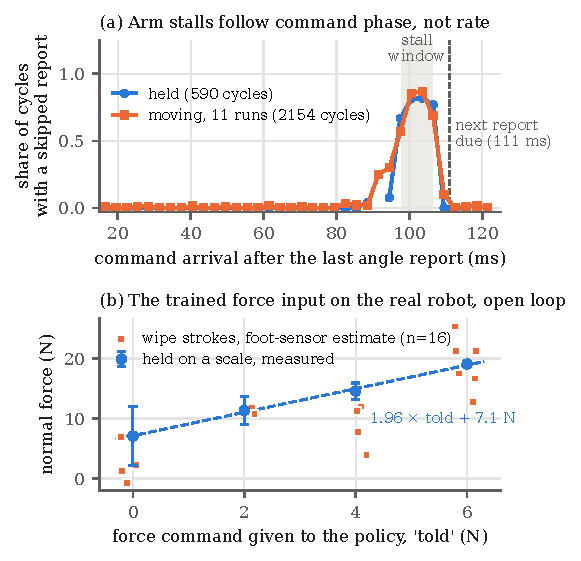
\includegraphics[width=\columnwidth]{figures/fig_interface_force.pdf}
\caption{(a) Share of report cycles followed by a skipped report, by where the latest command landed after the last
report (3\,ms bins). On a held arm at 5--10\,Hz, all 52 skips in 590 cycles had a command 88--110\,ms after the report;
none of 487 cycles without one skipped. (b) Real force under the hand on a scale (mean $\pm$ s.d.\ of 0.5\,s readings,
one run) and the foot-sensor estimate per wipe stroke (8 runs, 16 strokes), against the force command.}
\label{fig:interface}
\end{figure}

\textbf{\hyp{1}: stalls follow command phase.} The arm pauses its reports and its motion for 0.3--0.7\,s about every 2\,s
under a 10\,Hz stream. Fig.~\ref{fig:interface}a shows why. A command that lands 98--106\,ms after a report, just before
the next one is due, suppresses that report: at 10\,Hz, 36 of 42 such cycles skipped. A 100\,ms period drifts into this
window about once a second, then stays in it, because after a stall the next command lands in the window again. Locking
one command to each report (Table~\ref{tab:arm}) removed the stalls held and moving, and on the full six-joint motion
it cut the time lost from 29.7\% to 0.8\%. The worst joint error fell from 46$^\circ$ to about 10$^\circ$, and every
move ran on schedule. Under the locked stream, a first-order lag of 77\,ms behind a speed-limited target fits a
single-joint swing to 0.23$^\circ$ RMS (0.19--0.32$^\circ$ held out). The firmware-planner model we fitted earlier to large
steps does worse here (0.37$^\circ$). On the held-out six-joint motion with a payload, the model holds to
0.23--0.57$^\circ$ per joint.

\begin{table}[t]
\centering
\caption{Arm interface on hardware: free-running vs report-locked commands.}
\label{tab:arm}
\footnotesize
\setlength{\tabcolsep}{3pt}
\begin{tabular}{@{}lcc@{}}
\toprule
 & free-running & locked \\
\midrule
held, aimed at the window: skips & 53 / 56 & 0 / 716 \\
J1 swing at 36$^\circ$/s: skips & 73 / 710 & 1 / 894 \\
J1 swing: time lost & 29\% & $<$1\% \\
J1 swing: tracking RMS & 2.9--3.4$^\circ$ & 0.44--0.98$^\circ$ \\
six joints: skips & 46 / 390 & 2 / 449 \\
six joints: time lost & 29.7\% & 0.8\% \\
six joints: worst joint error & 46$^\circ$ & $\approx$10$^\circ$ \\
six joints: duration (plan 49.8\,s) & 54.6\,s & 50.2\,s \\
\bottomrule
\end{tabular}
\end{table}

\textbf{\hyp{2}: the idealized policy does not survive the interface.} Table~\ref{tab:policy} traces one policy lineage.
Scored on the fitted arm model, the policy trained on an idealized arm goes from 1.93 to 16.6\,cm median quiet goal error.
An earlier version of the arm model (the firmware planner fitted to large steps) shows the cause. There the policy
realized 0.28\,N of a 3.4\,N force command, and 87\% of its commands lay beyond a joint limit, a median 116$^\circ$ ahead
of the shoulder. On a stiff spring this acts as a push, but the firmware treats it as a place to go at 1.25\,rad/s.
Taken apart on that model, the 9--10\,Hz command rate alone costs 1.1--1.4\,cm, the 9\,Hz reports alone 2.1\,cm, and
the stiff servo alone 2.9\,cm. Together they cost more than the sum. Fine-tuning on the locked model recovered tracking (4.0\,cm) but shook the arm, with command steps of
10--14$^\circ$ RMS, half of them reversing. Tracking, falls and leg-chatter metrics all missed this. A penalty on the
delivered command step removed the shake and improved tracking with it, to 2.15\,cm.

\textbf{\hyp{3}: the legs did not respond as simulated.} That policy (\textsc{Step}) ran on the robot twice. Both runs
stopped at 1.5\,s on the arm-lead monitor, with J4's target 33--43$^\circ$ ahead of its report, where simulation
predicted 3.8$^\circ$. Over the handover the real legs moved 0.165 (rug) and 0.175 (wood) of their targets' motion. In
simulation the same measure is 0.51 without joint friction and 0.28--0.32 with 0.5--2\,N$\cdot$m. The cause of the
remaining gap is not identified. In simulation, holding the legs fixed reproduces the dependence: \textsc{Step} then reaches 13 of 27 goals
(median 7.5\,cm off), against 27 of 27 with the legs on the policy. The replay screen, built after the first failed run and not
fitted to the second, predicted the second run's J4 trajectory to 1.4$^\circ$ RMS (1.8$^\circ$ over all joints). We
retrained against friction-randomized legs with a wrist penalty (\textsc{Sticky}) and screened 16 checkpoints. None
passed both replay gates. The checkpoint we deployed was the nearest, missing the arm gate by 2--6$^\circ$. Deploying it
was a decision taken against our own pre-stated rule, to collect data, and we report it as such. On \textsc{Sticky}'s own
later runs, the replay ranked it correctly against \textsc{Step}. It was conservative on the stand (17--21$^\circ$ predicted
against at most 6.9$^\circ$ real in three of four runs). It did not reproduce the settled arm pose (10--11$^\circ$ RMS) and
under-predicted J4 on one far goal (13 against 23$^\circ$). It is a screen, not a forecast.

\begin{table}[t]
\centering
\caption{One policy lineage. Simulation: frozen validation set, quiet goal error (median / p90).
Hardware: hand by forward kinematics.}
\label{tab:policy}
\footnotesize
\setlength{\tabcolsep}{2.5pt}
\begin{tabular}{@{}p{0.215\columnwidth}p{0.29\columnwidth}p{0.45\columnwidth}@{}}
\toprule
policy & simulation & hardware \\
\midrule
\textsc{Ideal} & 1.93 / 2.57\,cm (own arm); 16.6 / 18.8\,cm (fitted arm) & not run: 87\% of targets beyond a joint limit \\
\textsc{Lock} & 4.02 / 4.90\,cm; steps 10--14$^\circ$ RMS & not run: shakes the arm \\
\textsc{Step} & 2.15 / 2.83\,cm; steps $\le$3.1$^\circ$ & 0 / 2 runs: lead stop at 1.5\,s \\
\textsc{Sticky} & far goals 60/60 clear of every stop, 3.0\,cm (1\,N$\cdot$m legs) & stand 4/4 (10\,s), 4.6--5.2\,cm; far goals 5/5 (incl.\ a 3-goal tour), 1.5--4.0\,cm; 30\,s walk, 3.1\,cm median, 6.9 worst; force wipes 8/8 \\
\bottomrule
\end{tabular}
\end{table}

\textbf{\textsc{Sticky} on hardware.} Across a stand, five far-goal runs (goals about 30\,cm from the start, radius
0.45--0.55\,m, up to 40$^\circ$ to the side), a 30\,s walk under joystick commands (to 0.28\,m/s and 0.46\,rad/s) and
13 bench wipes, no run was stopped by the robot's own monitors once the policy had taken over. Base tilt stayed below
10$^\circ$. One further wipe was refused at handover by the stance check, and two runs were ended by the operator
console's network watchdog, not by the robot. J4's lead is the remaining margin: it passed the
25$^\circ$ line twice for 0.18--0.24\,s in free air, under the 0.5\,s needed to stop. Sideways walking is barely tested
(1\,s).

\textbf{\hyp{4}: force.} With the hand goal set inside the scale's top, the policy stalled and pressed 18--26\,N whatever
the force command. Set at the scale's top, it pressed in proportion to the command (Fig.~\ref{fig:interface}b): 7.1 to
19.1\,N for 0 to 6\,N, about 2.0\,N per commanded newton. So the commanded value is not the delivered force, but it is
monotone. The foot-sensor sum, calibrated by the robot's weight alone, tracked the scale to 0.9\,N residual on a run it
was not fitted to. On eight bench wipes the estimated force rose with the command, about 2 to 21\,N, but varied from
$-4$ to 28\,N within a stroke, and the sensor zero drifted $\pm$9\,N with pose. Nothing regulated the force. Wiping
quality (area erased) is recorded on video but not yet scored.

%------------------------------------------------------------------------------
\section{Planned Experiments}
\label{sec:plan}

The Stage~2 plan tests each hypothesis on hardware against fixed baselines. Every trial is counted, aborts included. Hand
pose is measured externally (motion capture or a calibrated fixed camera with a tag on the gripper). All learned
results use three training seeds with fixed selection rules.

\textbf{E1 (\hyp{1}).} Locked against free-running streams at 5, 9, 10 and 11\,Hz, and at fixed phase offsets from 10 to
110\,ms, on all six joints, held and moving, and loaded at 0, 0.5 and 1\,kg. We will report skip rate and time lost
against phase. To test whether the phenomenon is specific to this unit, we will repeat the phase sweep on a second D1
unit, on the firmware and interface path that reports 40\,Hz \citep{schperberg2026safe} if it can be reproduced, and on
one other report-driven arm if we can get one.

\textbf{E2 (\hyp{2}).} On a frozen set of 20 goals per seed, standing, with external measurement, we compare
\textsc{Ideal} (deployed through the same Follower, behind the stop monitor), \textsc{Step}-recipe and
\textsc{Sticky}-recipe policies, and an \emph{ablation without the delivered-step penalty}. Measures: hand error
(median, p90), command-step RMS and reversals, and stops. \hyp{2} predicts that \textsc{Ideal} fails and that the real hand
error of the interface-trained policies lies within the simulated distribution. Model validity is tested separately by
predicting held-out logged trajectories at three speeds and under contact.

\textbf{E3 (\hyp{3}).} We take 8--12 checkpoints spanning the lineage and its seeds, chosen \emph{before} any of them is
run, and rank them two ways: by simulation metrics, and by the replay screen on a fixed library of recorded stands and
walks. All are then deployed on the same stand and far-goal protocol. The outcome is Spearman correlation of each ranking
with real arm lead, leg-target excursion and hand error. We also measure leg response against $k_p$ (20--40), a
friction identification with the legs lifted, and a leg-response randomization (scaling each leg's achieved motion)
against friction alone.

\textbf{E4 (\hyp{4}).} At five fixed poses and two surfaces with a force plate, we compare (i) open loop, (ii) an outer PI
loop on the foot-sensor estimate zeroed at the same pose, and (iii) a matched \emph{position-only} twin trained without
force inputs or force objectives, commanded by goal depth alone. Measures: force RMSE, peak, and contact loss. On
the wiping task we add erased area against a fixed pattern.

\textbf{E5 (whole-body against decoupled).} The vendor's locomotion controller with arm inverse kinematics, sent through
the same report-locked layer, on E2's goals and E4's wipes. If it matches the learned policy, the contribution is the
interface layer, not whole-body learning. In earlier simulation work on this robot, a decoupled door-opening controller
was competitive, so we treat this outcome as plausible.

%------------------------------------------------------------------------------
\section{Limitations}

The evidence so far comes from one robot, one training seed and few runs per condition. The hardware hand error is
computed, not measured. The leg-response gap is characterized but not explained. Friction accounts for part of it, and
the rest may be in the vendor's joint control or the real stance. The replay screen fixes the legs to their recorded
motion, so in principle it cannot evaluate a policy that would move the legs differently. E3 is designed to find out how
much this matters. The force results are open loop at one spot. The policy commands only position and force, and the
hand's orientation is left free.

%------------------------------------------------------------------------------
\section{Conclusion}

Low-cost arms make legged manipulation accessible, but they place the arm behind an interface that learned whole-body
methods do not model. Our preliminary evidence suggests the gap is set by command--report timing and by leg response
rather than by arm dynamics, and that both can be identified from the robot's own logs. The proposed experiments test
whether closing these interfaces is sufficient, whether a real-frame replay predicts deployment better than simulation,
and whether the learned whole-body policy is worth its cost over a decoupled controller with the same interface layer.

\bibliographystyle{plainnat}
\bibliography{references}

\end{document}
